\chapter{Ansatz}\label{ch:ansatz}
Before we delve into details let us preface this section with an etymology of the word ansatz. An ansatz is a term borrowed from German (plural ansätze), referring to an educated guess, an initial point, or an additional assumption made to facilitate solving a problem, which may later be verified based on the results obtained~\cite{ansatz_etymology}.

In the context of quantum computing, an ansatz refers to a parametrized quantum circuit, which is comprised of quantum gates and some of them are parametrized. Ansatzes are often used in variational algorithms where the circuit parameters are optimized by classical computers.

In this chapter, we will discuss the role of the ansatz, its properties, types, and introduce several popular examples. Moreover, we will address the challenges that can impede the design of an ansatz.

\section{Expressibility}
The notion of expressibility can be very helpful to get an understanding what is the role of the ansatz. Expressibility says how much of the Hilbert space can be covered by our ansatz. The following images should provide a clear explanation of this idea.

\begin{figure}[H]
        \centering
        \begin{minipage}{0.4\linewidth}
            \centering
            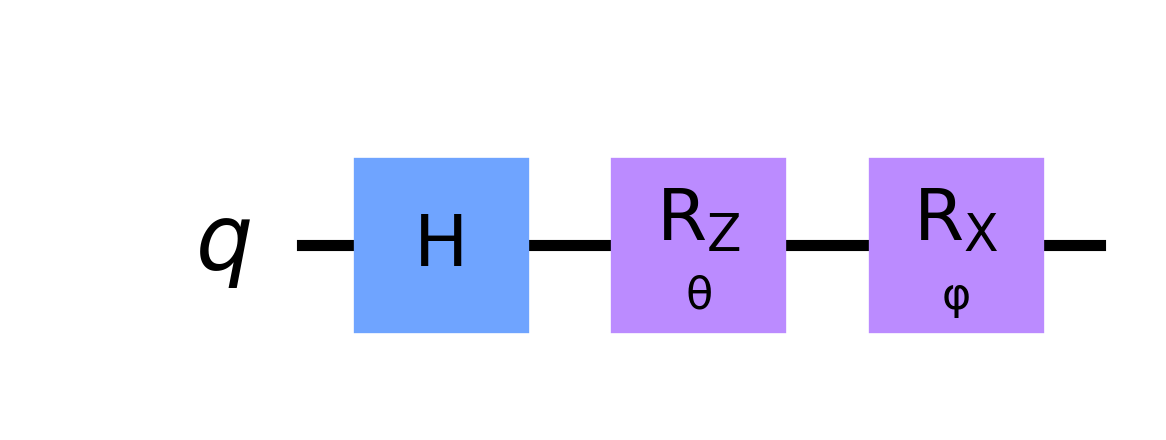
\includegraphics[scale=0.9]{expressibility-hrzrx-circuit.png}
        \end{minipage}
        \begin{minipage}{0.4\linewidth}
            \centering
            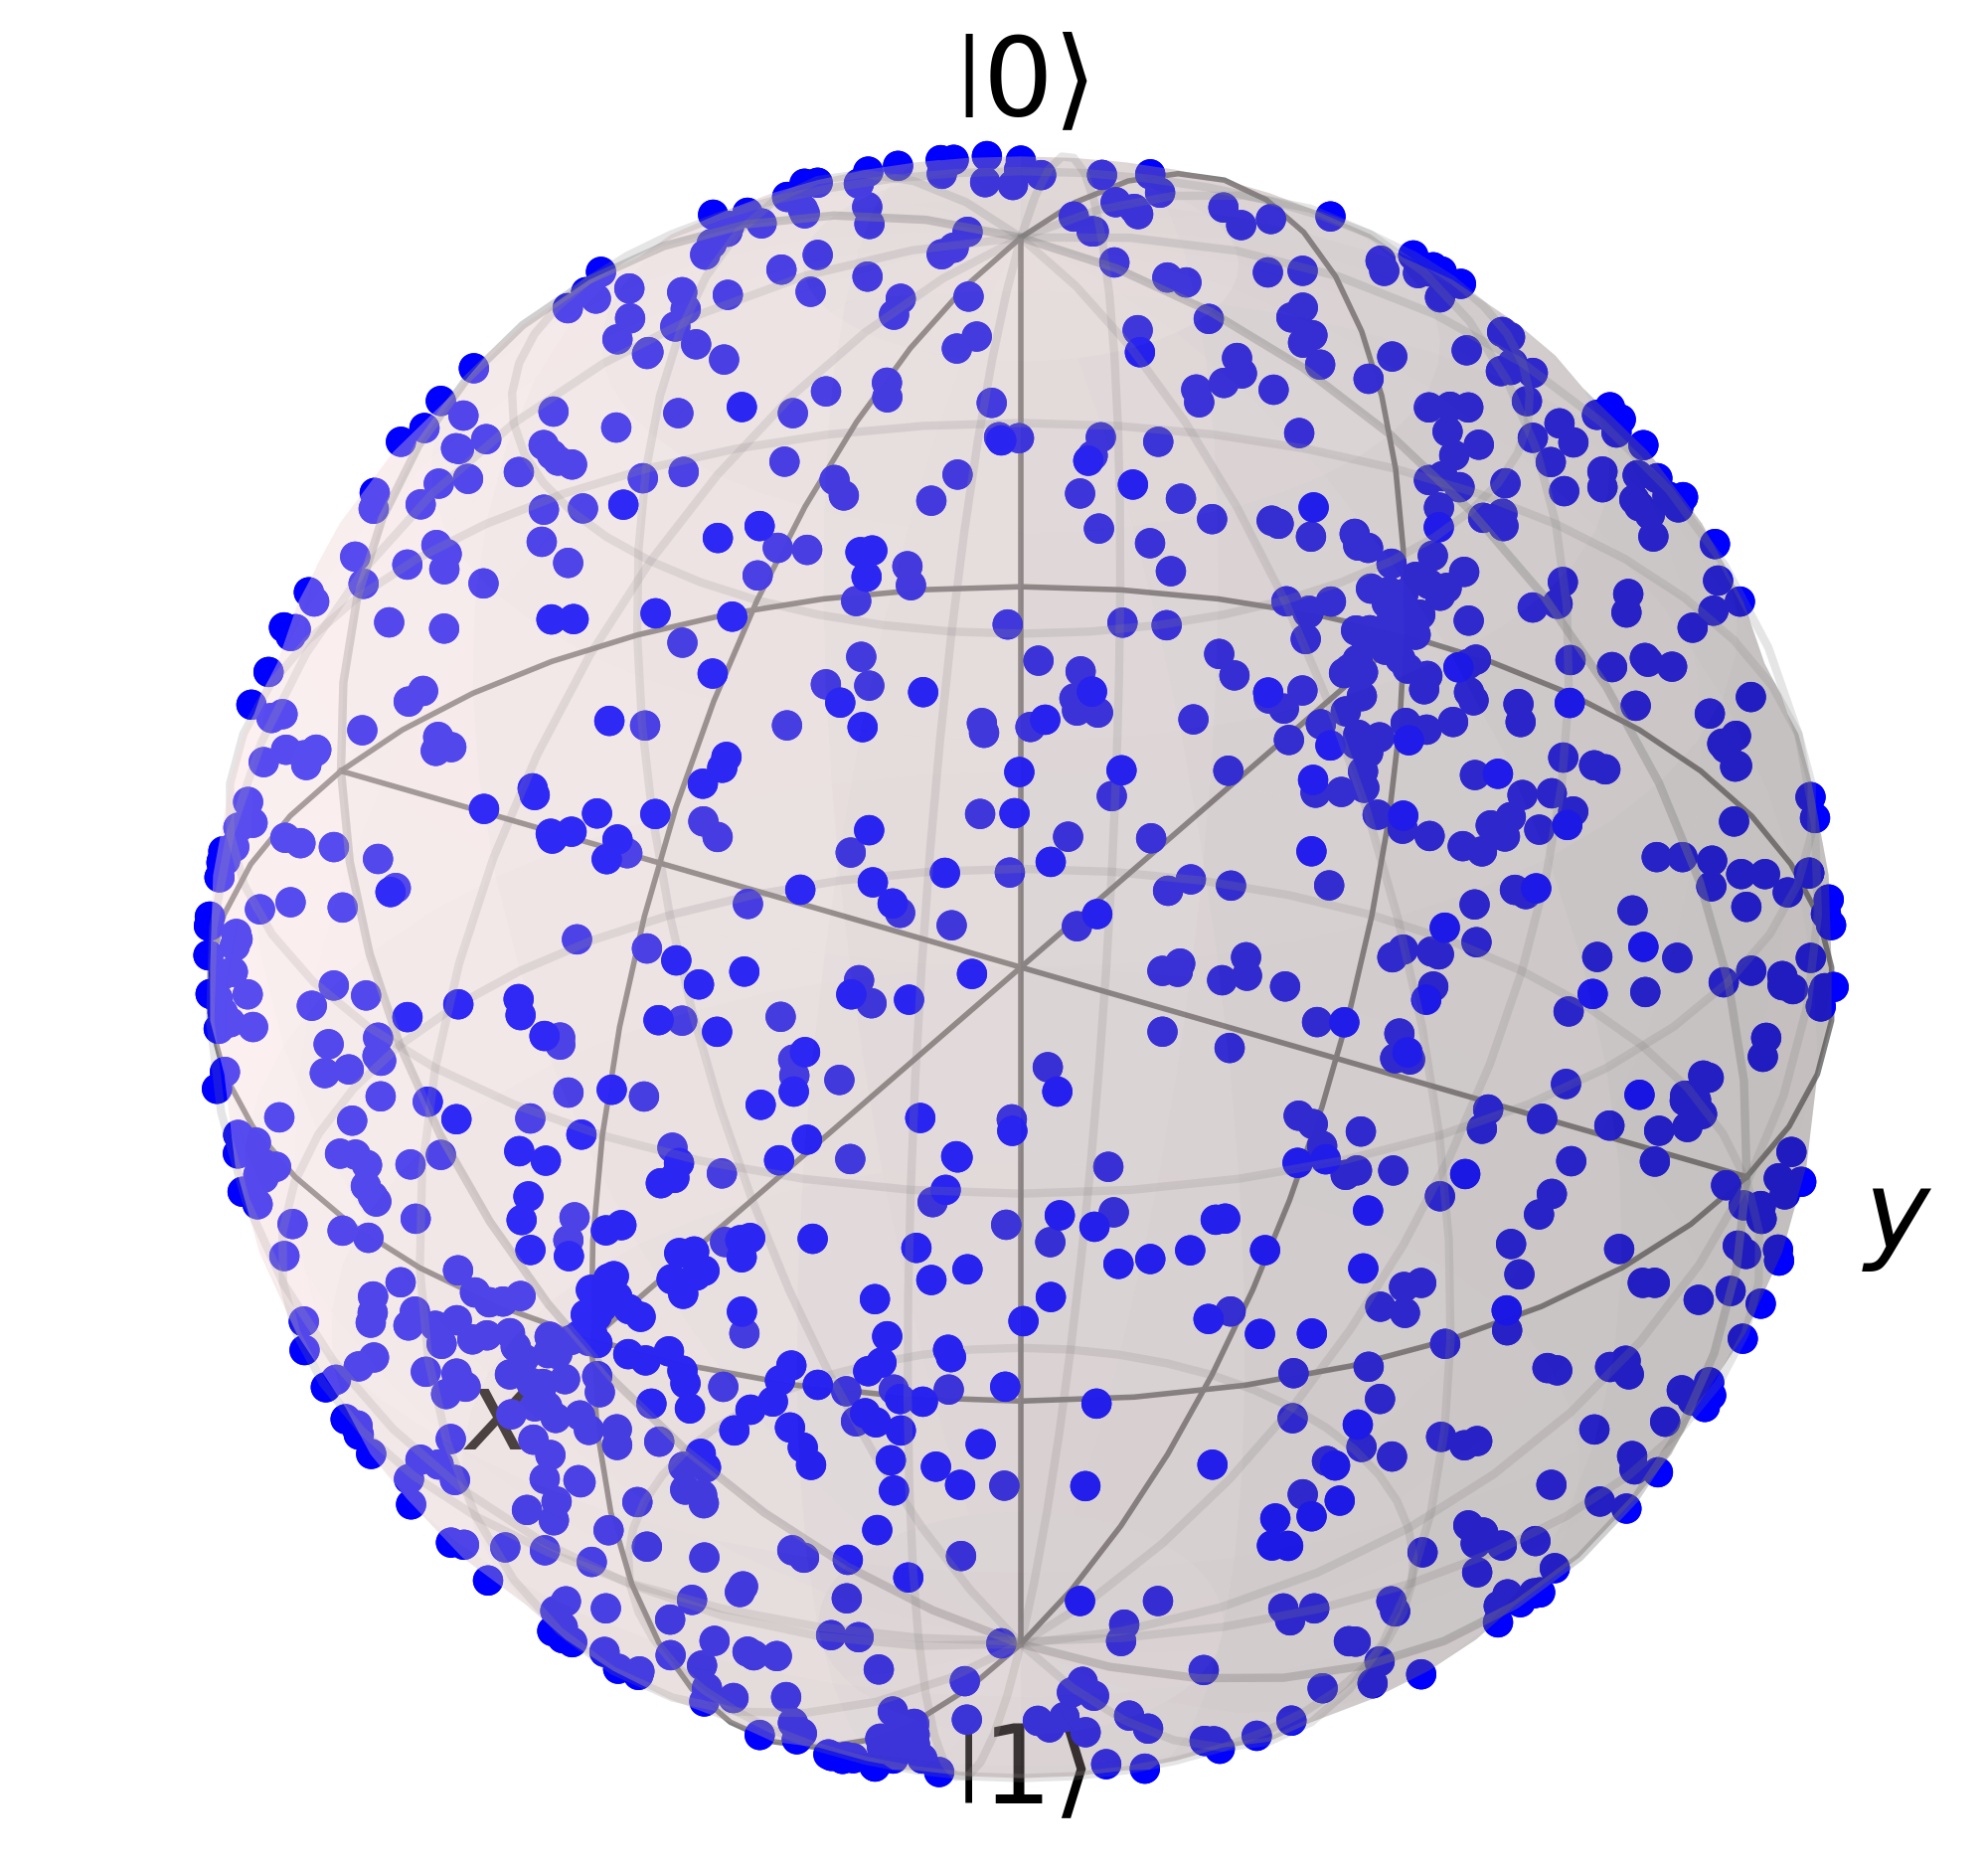
\includegraphics[scale=0.42]{expressibility-hrzrx-qubit.png}
        \end{minipage}
        \caption{Ansatz expressibility, 1000 parameters sampled uniformly randomly}
\end{figure}

Provided we know that our solution is a real number, we can use a simpler ansatz that covers only a real part of the Hilbert space. Additional gates would introduce more noise into our circuit and the more parameters we have, the more difficult it is to optimize them.

\begin{figure}[H]
    \centering
    \begin{minipage}{0.4\linewidth}
        \centering
        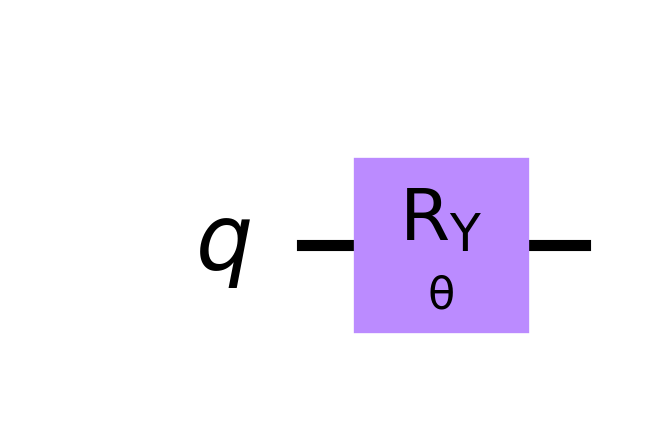
\includegraphics[scale=0.95]{expressibility-ry-circuit.png}
    \end{minipage}
    \begin{minipage}{0.4\linewidth}
        \centering
        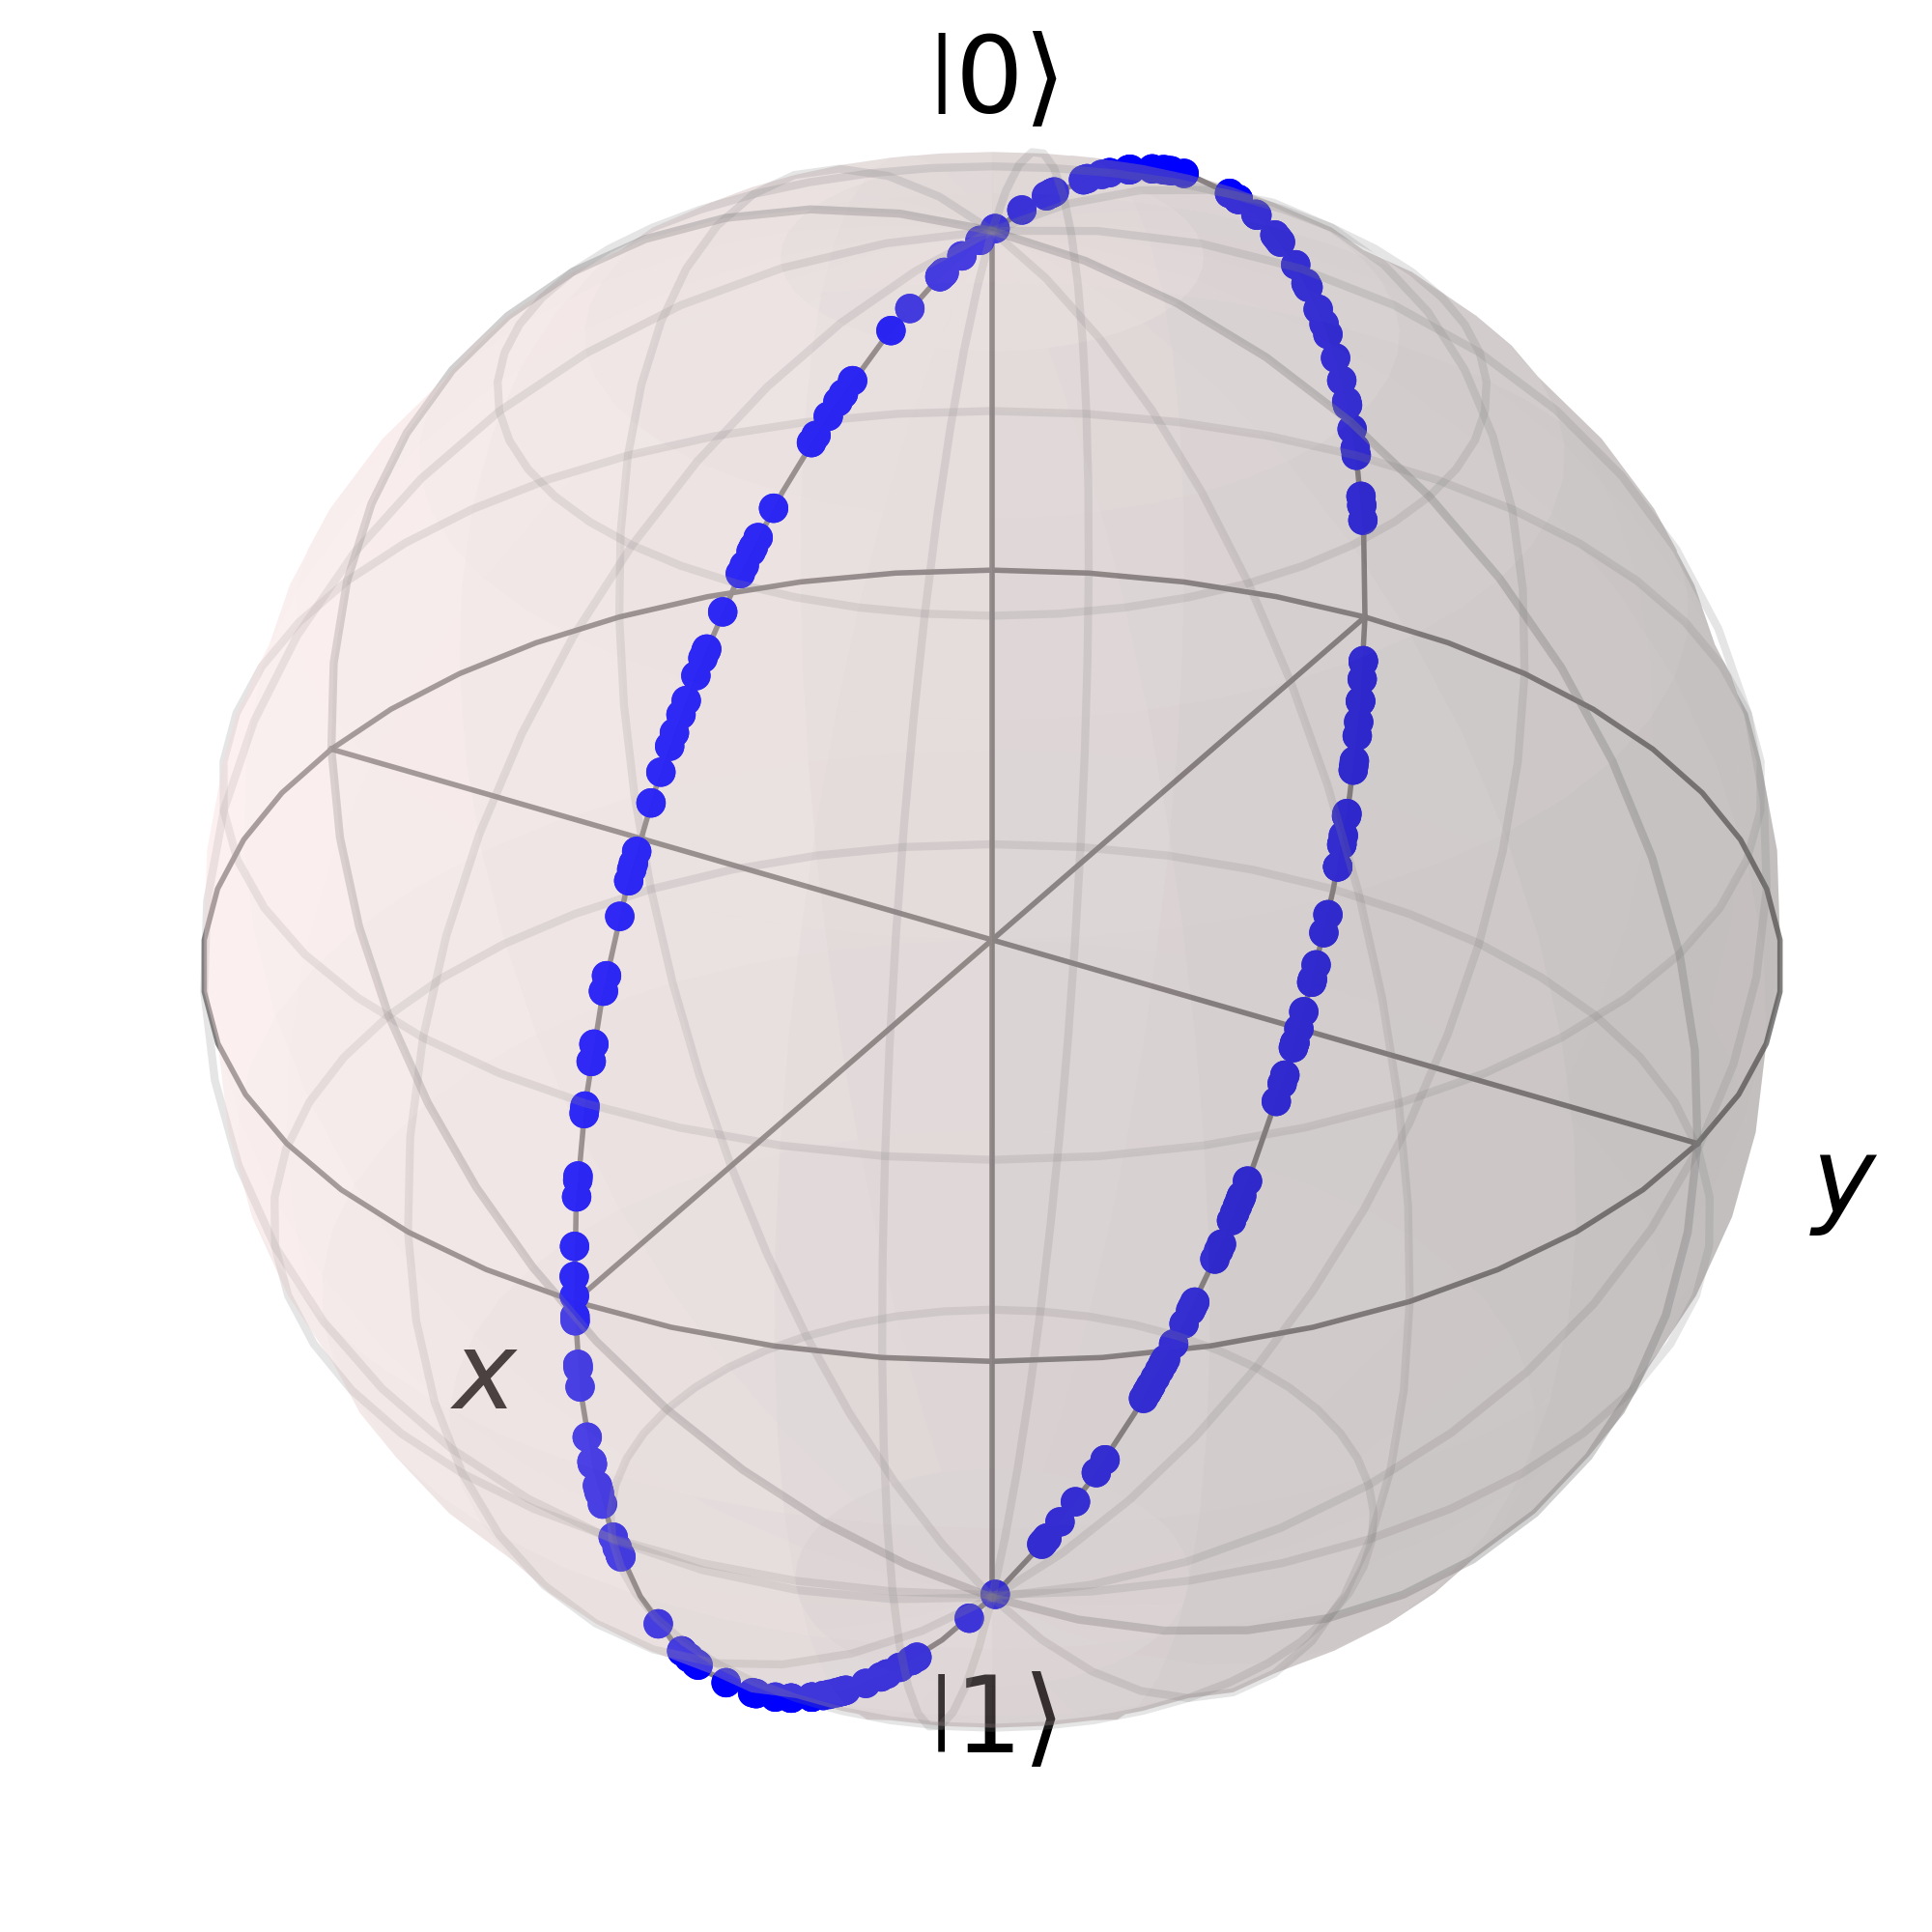
\includegraphics[scale=0.42]{expressibility-ry-qubit.png}
    \end{minipage}
    \caption{Ansatz expressibility, 200 parameters sampled uniformly randomly}
\end{figure}

\section{Trainability}
The trainability of an ansatz denotes its ability to efficiently optimize its parameters, typically through iterative processes. A major hurdle that can impede the trainability of an ansatz is the barren plateau problem (vast planes in cost function) which we will introduce in the following chapter. Holmes et al.~\cite{holmes2022} claim that trainability and expressibility are inversely related. Furthermore, they claim that highly expressive ansätze are more prone to barren plateaus and therefore are harder to train, however, that does not necessarily mean that inexpressive ansatzes cannot have trainability issues. The priority should be to span only the relevant part of the Hilbert space, ideally only where the solution lies and minimize the number of parameters and gates that can introduce noise. Designing an efficient ansatz involves finding an optimal trade-off between expressibility and trainability~\cite{holmes2022}.

\ques{barren plateau is defined in the next chapter, should I move it somewhere before this trainability? sometimes it is difficult the figure out the right positioning since the topics are interconnected}

\section{Circuit depth}
A circuit depth is a measure that says how many ``levels'' of gates a quantum circuit contains. Alternatively, we can say it is the longest path in a circuit. It is a way to increase expressibility but at the same time is a way how to introduce more noise into a circuit.

\begin{figure}[H]
    \centering
    \begin{subfigure}[b]{0.2\textwidth}
        \centering
        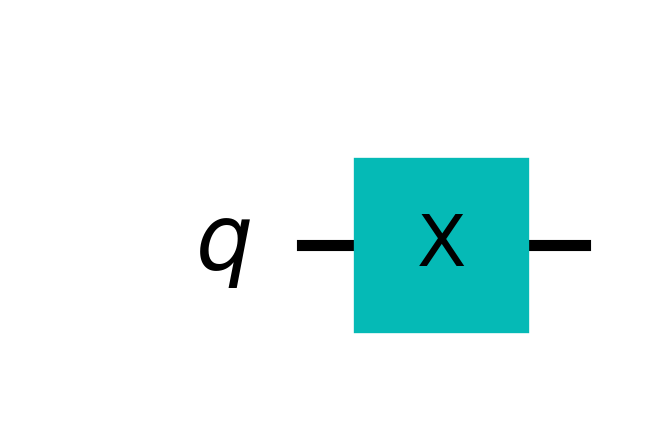
\includegraphics[scale=0.7]{circuit-depth-1.png} 
        \caption*{1}
    \end{subfigure}
    \hfill
    \begin{subfigure}[b]{0.3\textwidth}
        \centering
        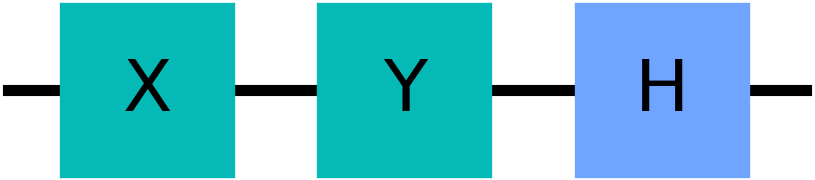
\includegraphics[scale=0.7]{circuit-depth-3.png}
        \caption*{3}
    \end{subfigure}
    \hfill
    \begin{subfigure}[b]{0.45\textwidth}
        \centering
        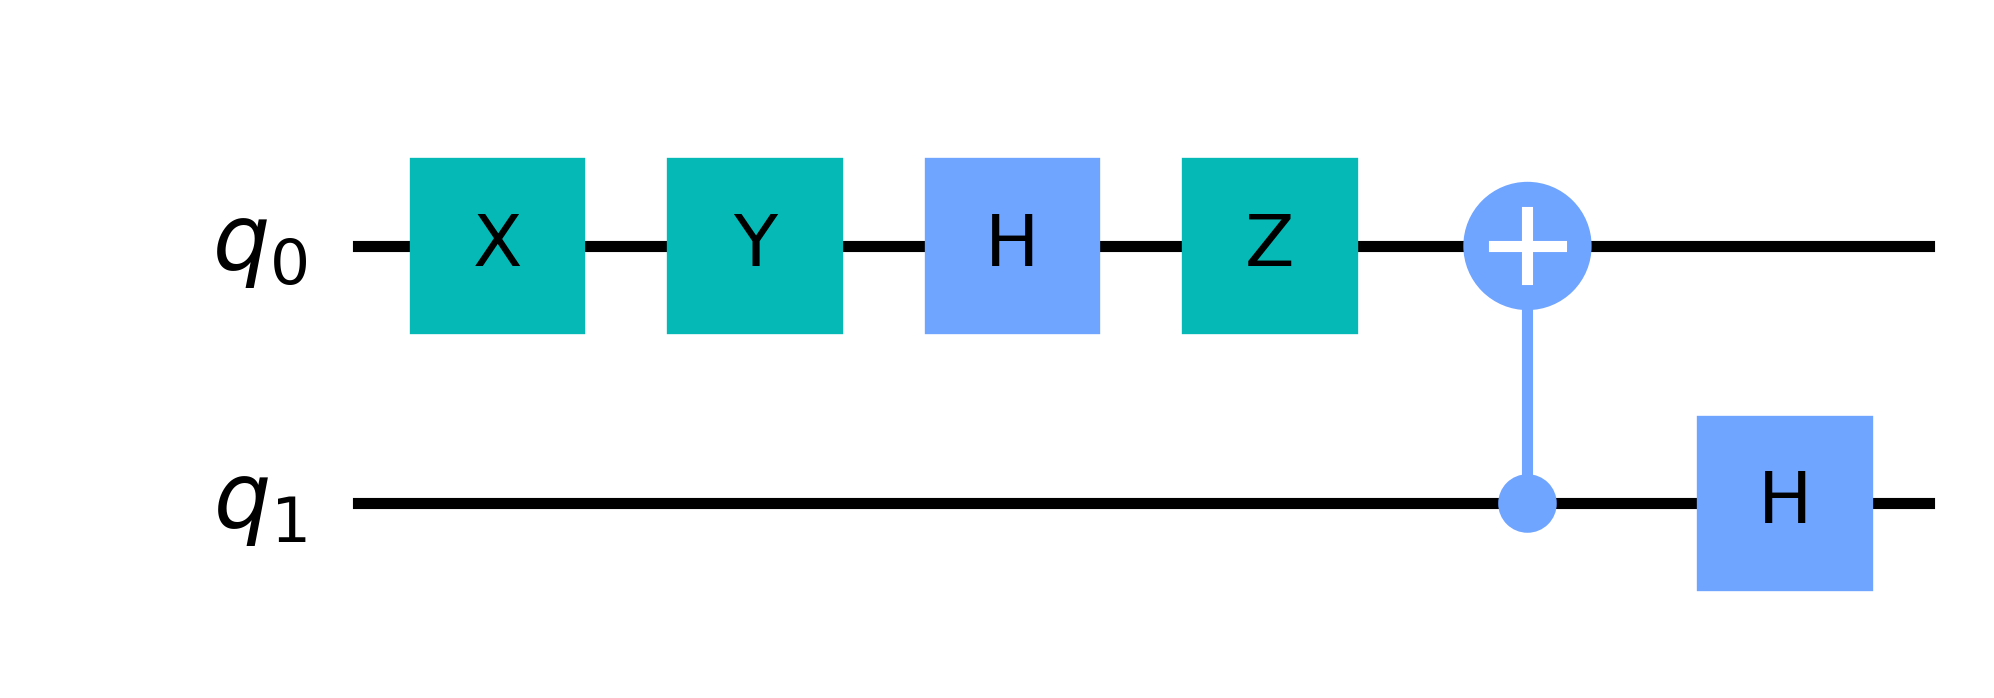
\includegraphics[width=\textwidth]{circuit-depth-6.png}
        \caption*{6}
    \end{subfigure}
       \caption{Circuit depth}
       \label{fig:circuit-depth}
\end{figure}

\section{Types of ansatzes}
There is a plethora of ansatzes, yet we will focus only on the most popular approaches. Broadly we can classify them into two categories, problem-inspired and hardware-inspired. In addition to that, if ansatz leverages a structure of a particular problem, is said to be problem-specific/problem-derived, otherwise it is problem-agnostic/general. 

\subsection{Hardware efficient ansatz (HEA)}
A problem-agnostic ansatz designed with hardware constraints in mind. The goal is to minimize the number of circuit depth, the number of gates, and entangling qubits in such a way it can be easily implemented on real hardware and thereby tries to minimize error, noise and decoherence. The fact whether an ansatz is hardware efficient heavily depends on the hardware we are using. This will be briefly discussed in the next subsection.

The structure of HEA consists of layers, each layer consists of rotation gates and entangling gates. In a single layer, we can add multiple levels of rotations using different gates. The final layer does not contain any entangling gates, only rotation gates. 

\begin{figure}[H]
    \centering
    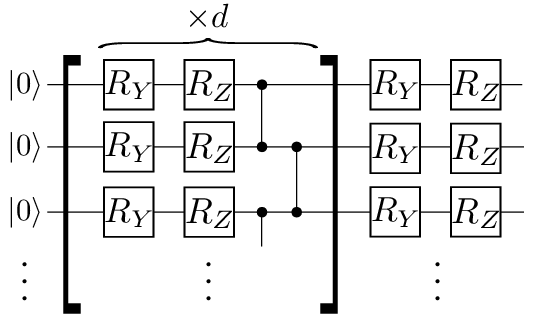
\includegraphics[width=0.5\textwidth]{hea-structure.png}       
    \caption{Hardware efficient ansatz structure~\cite{img:hea}}     
\end{figure}
The main drawback of hardware efficient ansatzes is that they can span a substantial portion of the Hilbert space, often exceeding what is necessary~\cite{holmes2022}. This results in barren plateaus and also when dealing with a large number of parameters classical optimizers face increased challenges in their optimization task. There is ongoing research about ansatzes, there is an article that claims to have trainability guarantees for hardware efficient ansatzes that possess specific properties~\cite{shallow}. Nevertheless, we cannot be certain about that. Other research endeavors attempted to disrupt this theory by introducing a new source of untrainability~\cite{hea-practical}.

\subsubsection{Qubit topology and transpilation}
To deepen understanding and foster motivation for a hardware-efficient ansatz, we will explore the specifics of IBM hardware in more detail. IBM has many quantum computers with various qubit counts, topologies, and native gate sets. A qubit topology shows qubit connectivity. Upon observation of the qubit topology depicted in Figure \ref{fig:qubit_topology}, it becomes apparent that certain qubits are disconnected and situated far from one another. One might ask how to implement a two-qubit gate between these qubits. The process is outlined in the IBQ documentation~\cite{transpiler,native_gates}, but in brief, it can be summarized as follows.

To apply a 2-qubit gate to a quantum circuit between qubits that are not directly connected on a quantum computer, it is necessary to incorporate one or more swap gates into the circuit. These swap gates facilitate the rearrangement of qubit states until they are positioned adjacent to each other on the device gate map. Each swap gate is both a noisy and expensive operation to perform. Determining the minimum number of swap gates needed to align a circuit with a device is crucial. However, finding the optimal swap mapping is challenging as this problem belongs to the NP-hard problems, making it expensive to compute for larger quantum devices. Qiskit defaults to using a stochastic heuristic algorithm to compute a satisfactory swap mapping.

Moreover, besides connectivity issues, compatibility with the hardware's native gate set must be addressed. Each processor family operates with its own set of native gates. By default, these systems only support operations within their respective gate sets. Consequently, every gate in the circuit needs to be translated into elements of this set. This process is called circuit transpilation and Qiskit provides multiple optimization levels The higher the level is, the more difficult it is to compute that but it may result in a more optimal circuit. Fortunately, it is handled automatically by Qiskit so we do not have to worry about it. 

\begin{figure}[H]
    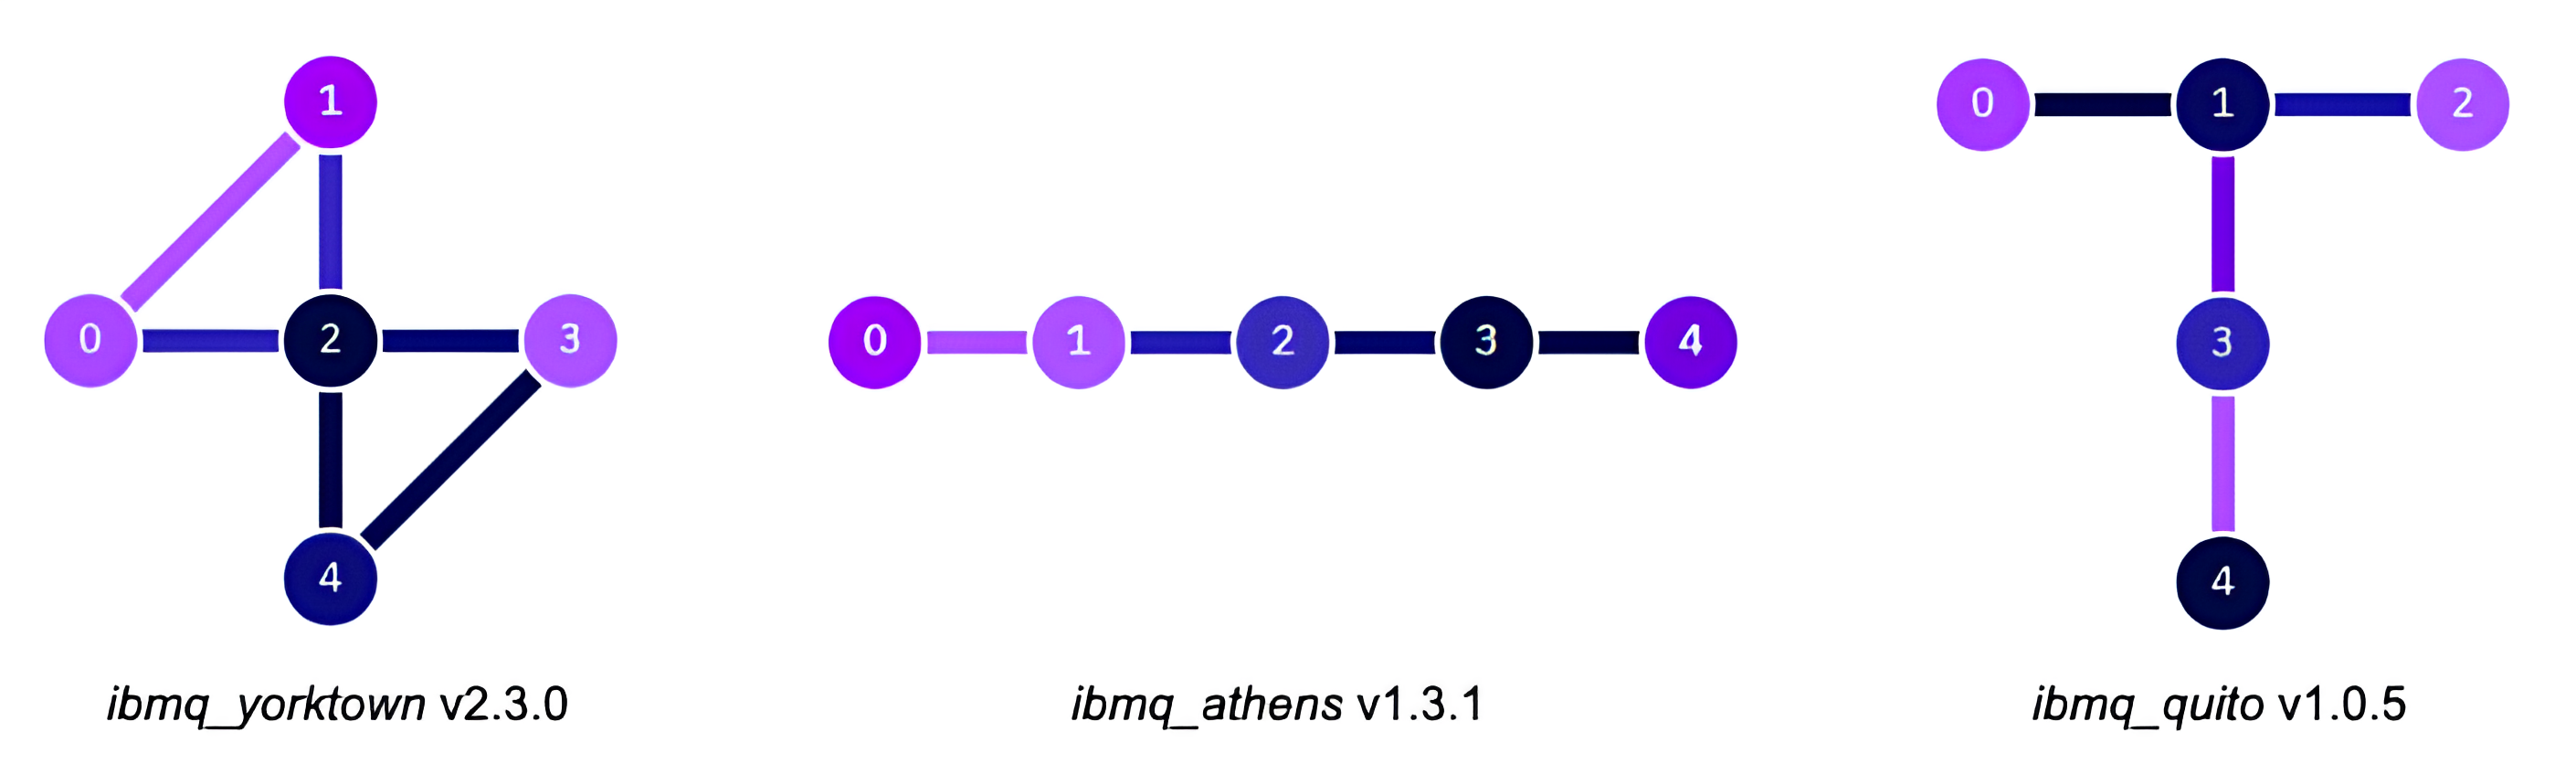
\includegraphics[width=\linewidth]{qubit-topology.png}
    \caption{Example qubit topology of IBM quantum computers~\cite{img:topology}}
    \label{fig:qubit_topology}
\end{figure}

\subsection{United Coupled Cluster (UCC)}
Unlike HEA, this type of ansatz does not take into account any hardware constraints. It is a chemistry-inspired ansatz proposed for finding a ground state energy of molecules. Despite it being chemistry-inspired, it is still a problem-agnostic ansatz. While this appears favorable, it suffers from a major drawback. A circuit depth of UCC ansatz grows $O(n^4)$ where $n$ is a number of qubits~\cite{ucc_ansatz}. For larger problems and current NISQ devices, this is not feasible due to noise and decoherence, although there is ongoing research to mitigate this problem.
  
\subsection{Popular ansatzes}
This section will introduce several popular ansatzes categorized by type of entanglement. All the ansatzes come from IBM Quantum documentation~\cite{twolocal}. 

\subsubsection{Full entanglement}
This ansatz entangles each qubit with every other qubit, therefore we can hardly name this ansatz as hardware efficient.
\begin{figure}[H]
    \centering
    
\includegraphics[width=\linewidth]{full-ansatz.png}
    \caption{Full entanglement ansatz, 2 layers, RY rotation gates}
\end{figure}

\subsubsection{Linear entanglement}
In this ansatz, each qubit is entangled with the next qubit. 
\begin{figure}[H]
    \centering
    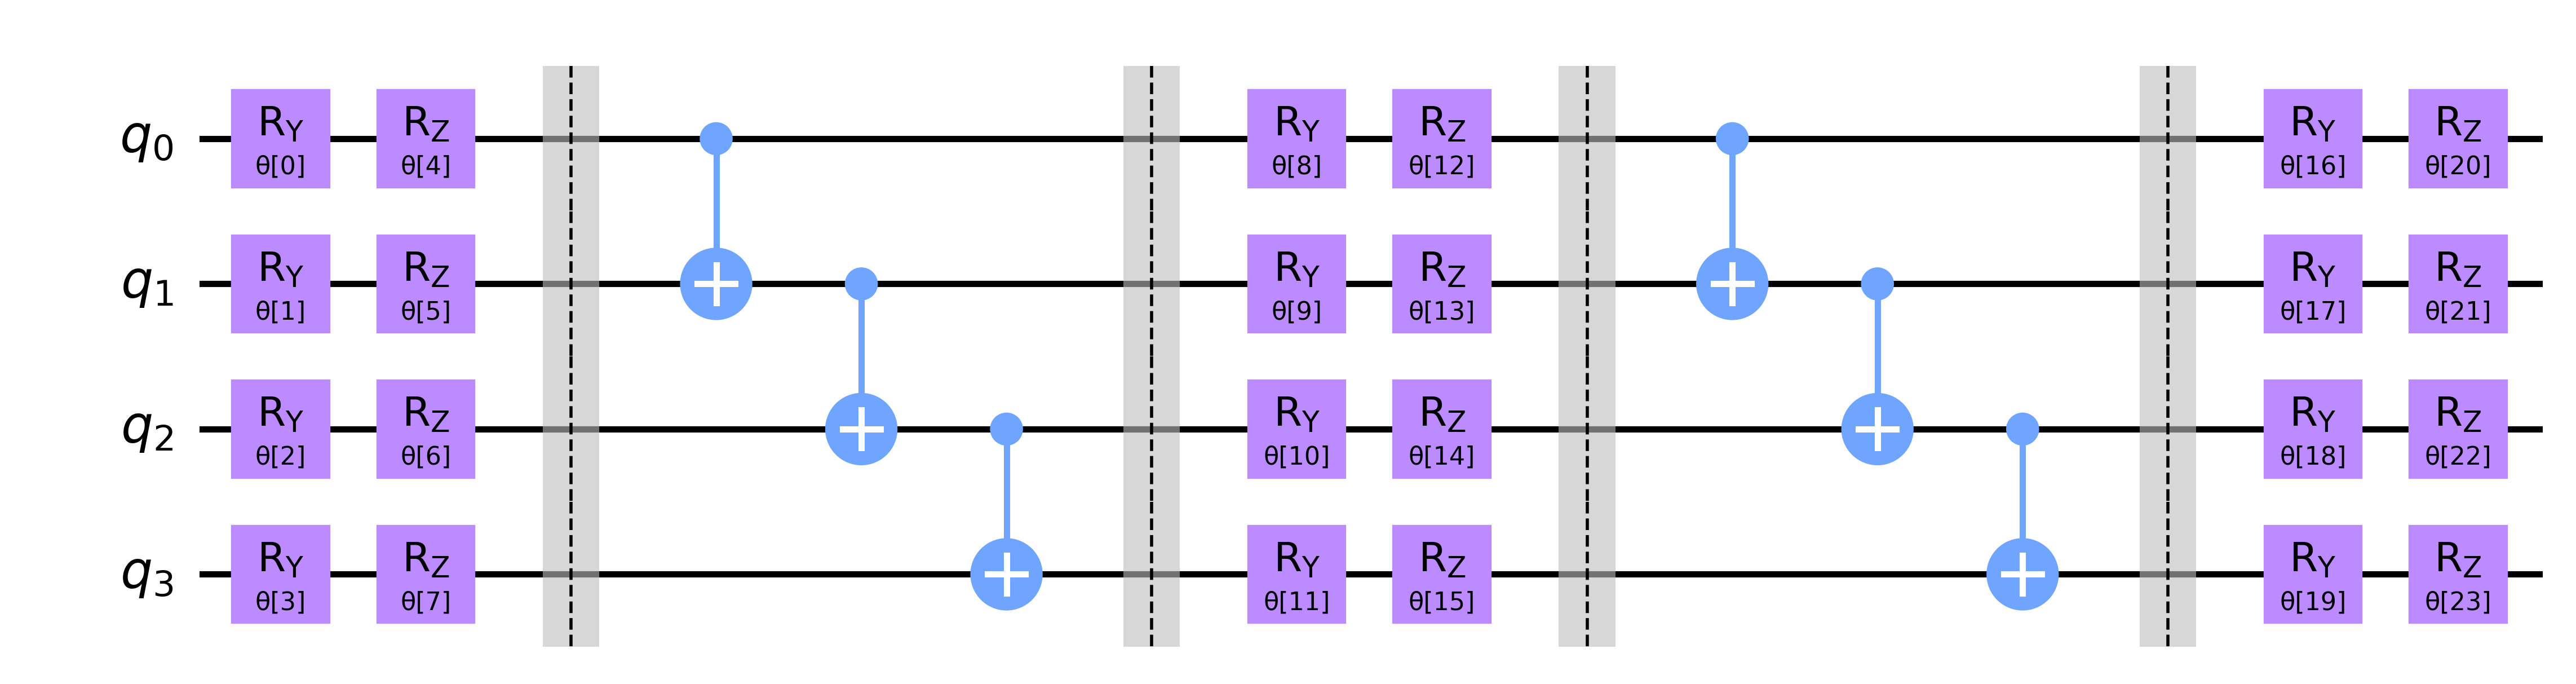
\includegraphics[width=\linewidth]{linear-ansatz.png}
    \caption{Linear entanglement ansatz, 2 layers, RY rotation gates}
\end{figure}

\subsubsection{Reverse linear entanglement}
As the name suggests, this is the linear ansatz just in a reversed order. Provided the entangling gates are CNOTs, this ansatz has the same unitary matrix as the full entanglement. 
\begin{figure}[H]
    \centering
    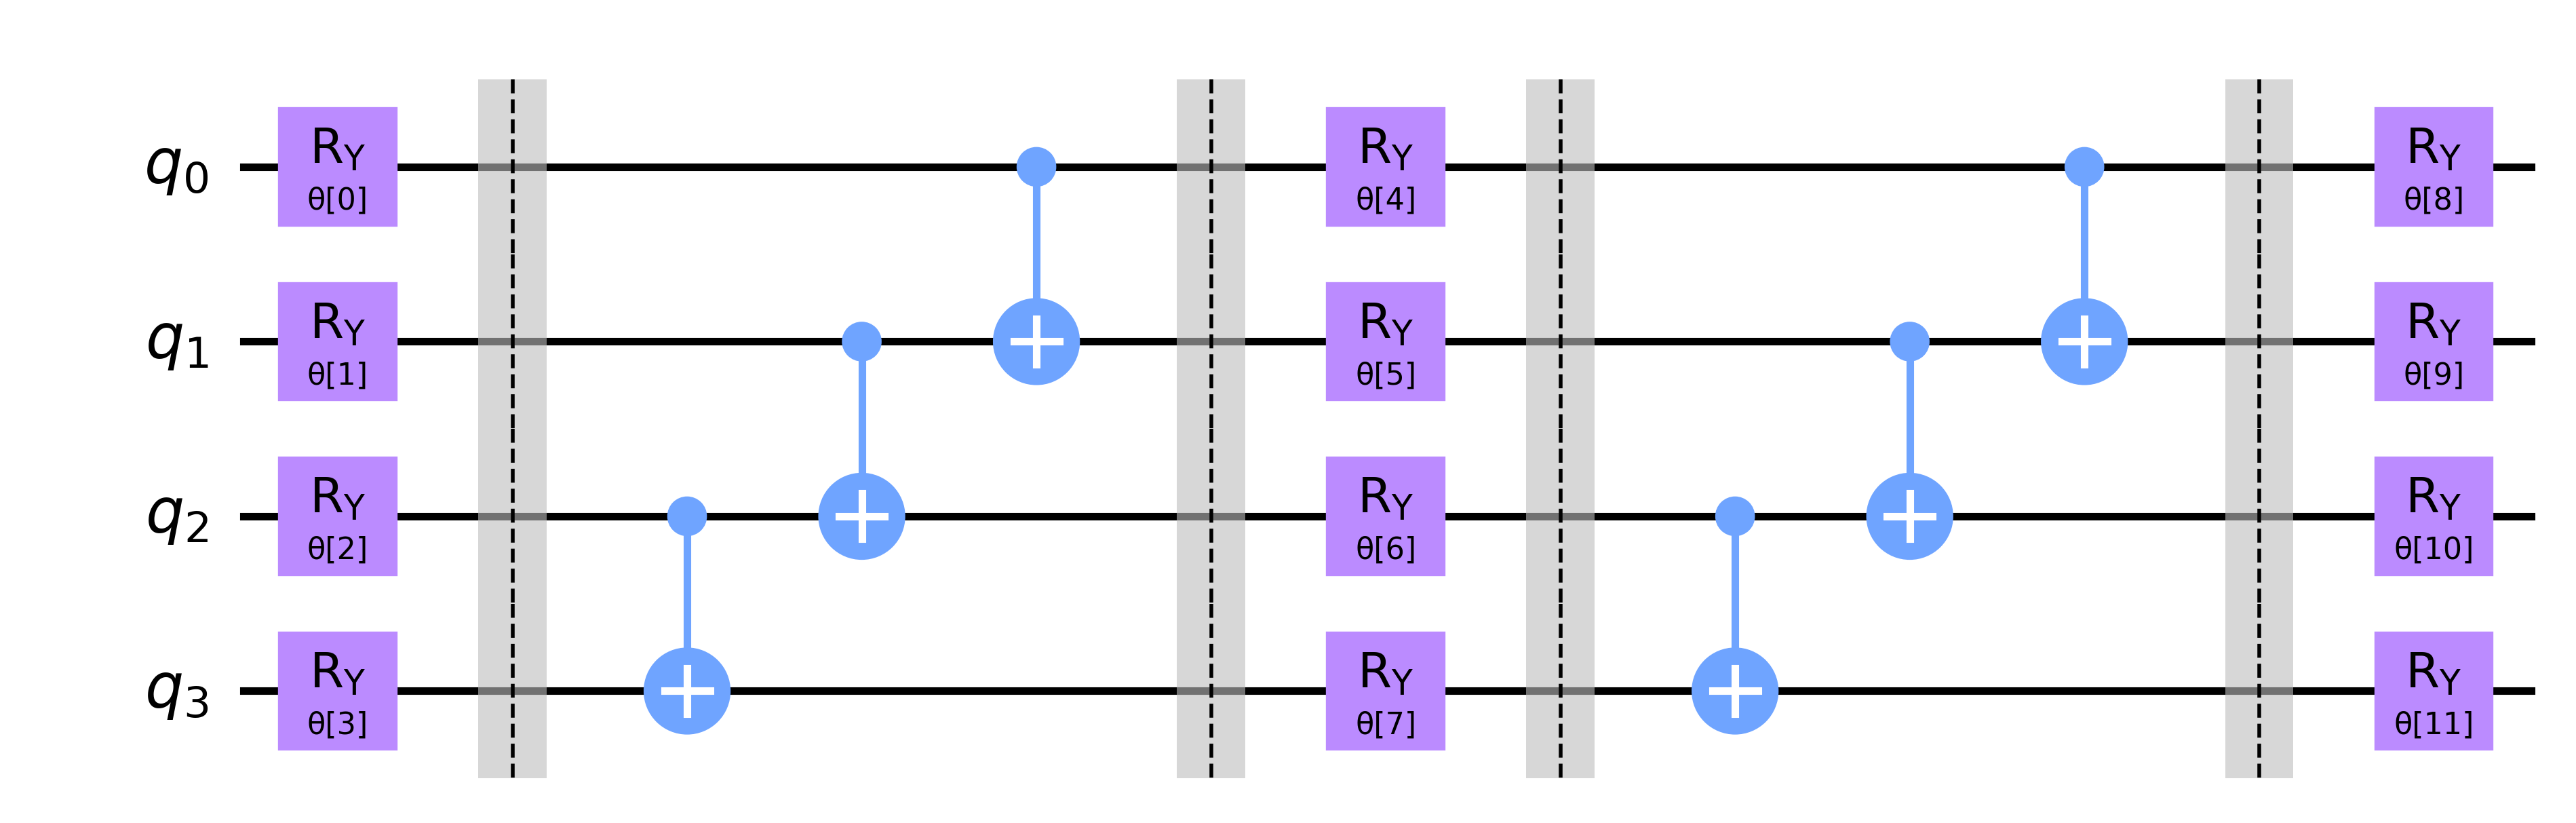
\includegraphics[width=\linewidth]{reverse-linear-ansatz.png}
    \caption{Linear entanglement ansatz, 2 layers, RY rotation gates}
\end{figure}

\subsubsection{Pairwise entanglement}
The entanglement layer consists of two ``levels''. In the first level, qubit $i$ is entangled with qubit $i+1$ for all even values of $i$, and then in the second level qubit $i$ is entangled with qubit $i+1$ for all odd values of $i$. 
\begin{figure}[H]
    \centering
    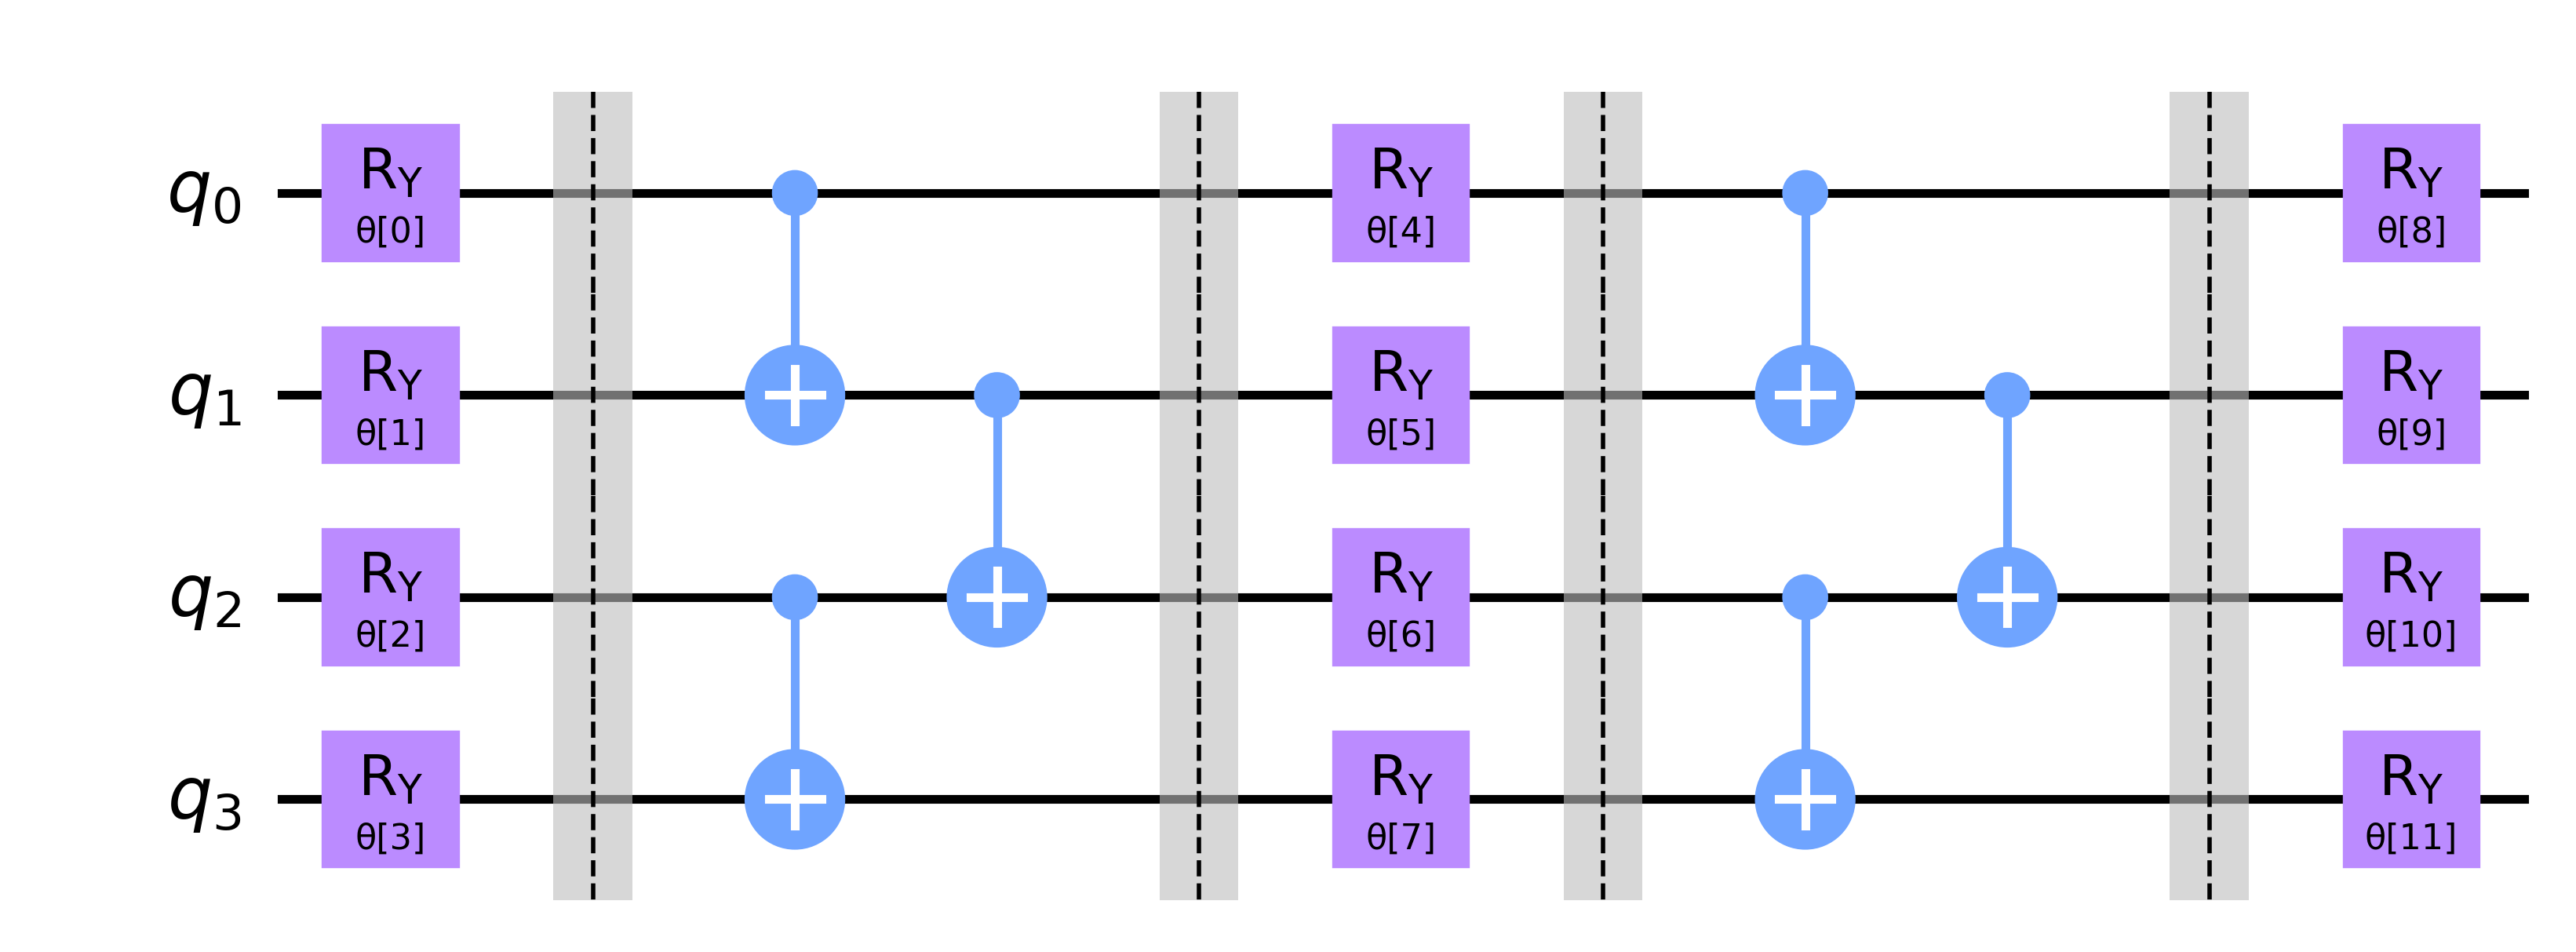
\includegraphics[scale=0.7]{pairwise-ansatz.png}
    \caption{Pairwise entanglement ansatz, 2 layers, RY rotation gates}
\end{figure}

\subsubsection{Circular entanglement}
This is an extension of the linear entanglement where the last qubit is also entangled with the first qubit. In case physical qubits are arranged into a circle, it is easy to implement.
\begin{figure}[H]
    \centering
    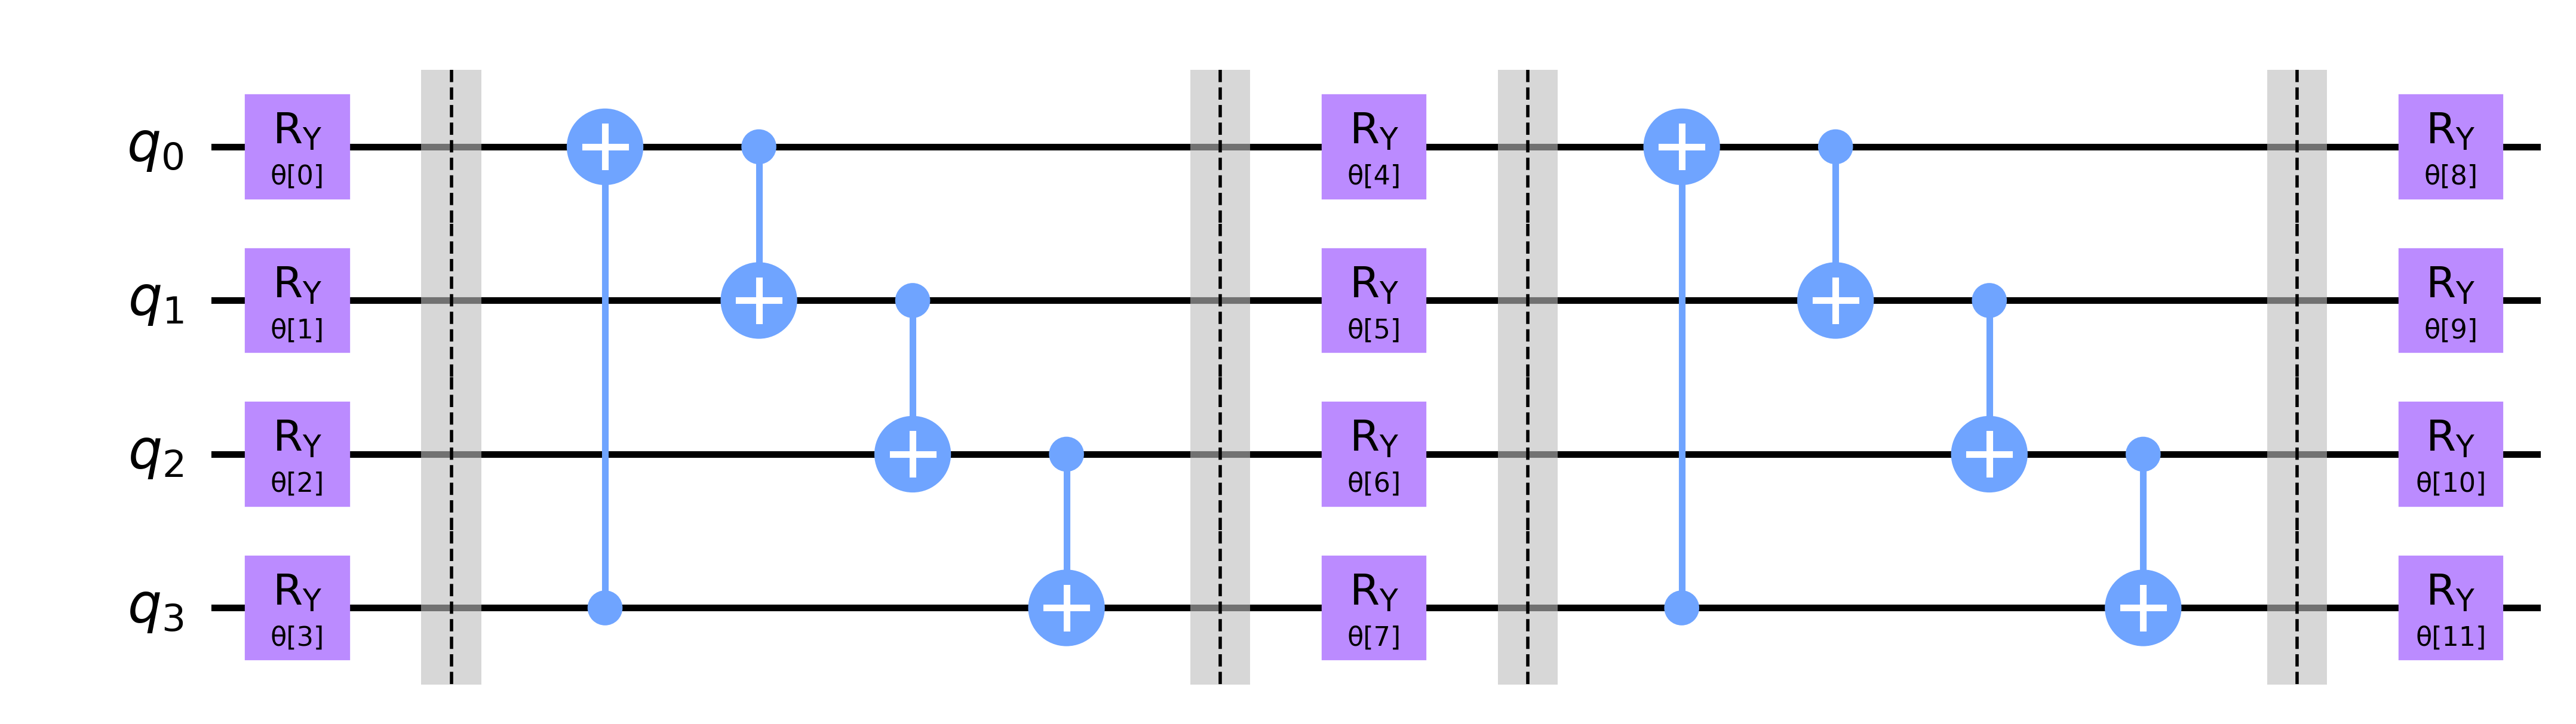
\includegraphics[width=\linewidth]{circular-ansatz.png}
    \caption{Circular entanglement ansatz, 2 layers, RY rotation gates}
\end{figure}

\subsubsection{Shifted circular alternating (SCA) entanglement}
SCA entanglement ansatz consists of circular entanglement where the entangling gate connecting the first with the last qubit is shifted by one in every layer. Furthermore, the role of control and target qubits are swapped in every layer (therefore alternating).
\begin{figure}[H]
    \centering
    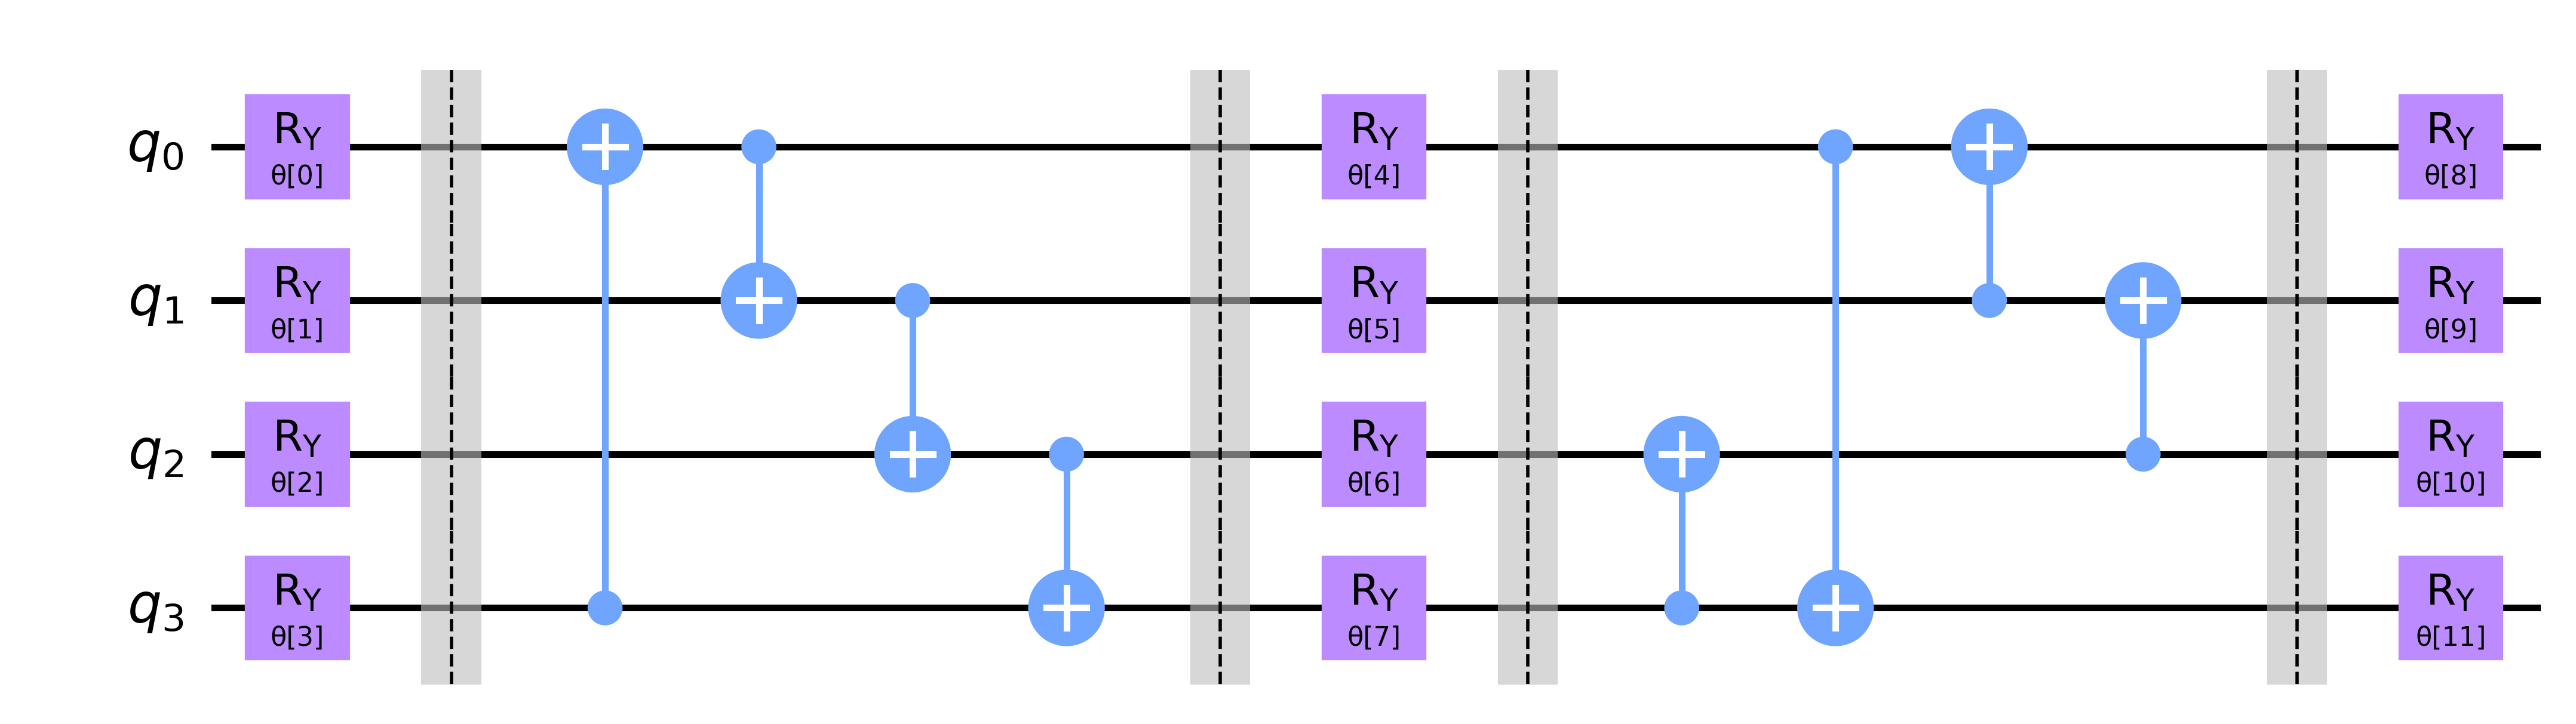
\includegraphics[width=\linewidth]{sca-ansatz.png}
    \caption{Shifted circular alternating entanglement ansatz, 2 layers, RY rotation gates}
\end{figure}